\documentclass[tikz]{standalone}
\usepackage{amsmath}
\usepackage{tikz}

\begin{document}

\begin{figure}[h]
\begin{center}
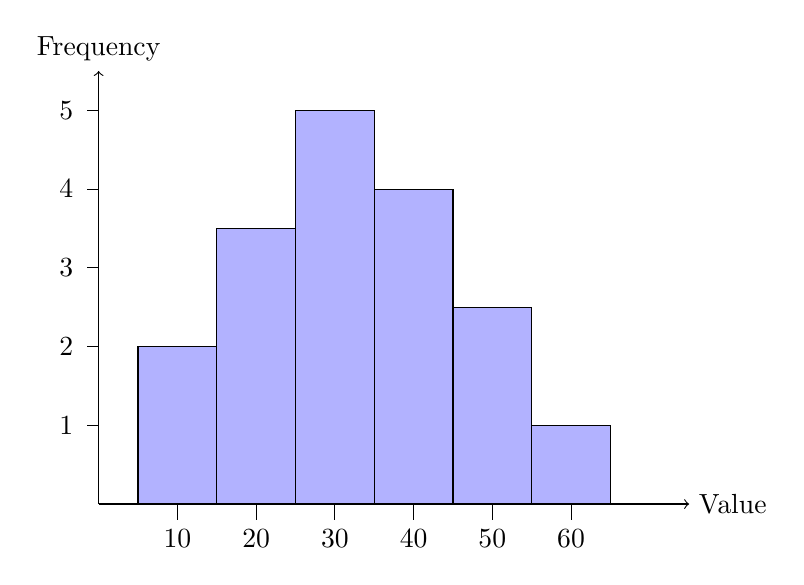
\begin{tikzpicture}
  \draw[->] (0,0) -- (7.5,0) node[right] {Value};
  \draw[->] (0,0) -- (0,5.5) node[above] {Frequency};

  \filldraw[fill=blue!30] (0.5,0) rectangle (1.5,2);
  \filldraw[fill=blue!30] (1.5,0) rectangle (2.5,3.5);
  \filldraw[fill=blue!30] (2.5,0) rectangle (3.5,5);
  \filldraw[fill=blue!30] (3.5,0) rectangle (4.5,4);
  \filldraw[fill=blue!30] (4.5,0) rectangle (5.5,2.5);
  \filldraw[fill=blue!30] (5.5,0) rectangle (6.5,1);

  \foreach \x/\label in {1/10, 2/20, 3/30, 4/40, 5/50, 6/60} {
    \draw (\x,0) -- (\x,-0.2);
    \node[below] at (\x, -0.2) {\label};
  }

  \foreach \y in {1,...,5} {
    \draw (0,\y) -- (-0.15,\y);
    \node[left] at (-0.2,\y) {\y};
  }
\end{tikzpicture}
\end{center}
\caption{An illustration of histogram.}
\end{figure}

\end{document}